\documentclass[UTF8]{ctexart}

\title{电子技术基础实验第十三周实验报告}

\author{王磊\quad2022012972}

\date{\today}

\usepackage{geometry}
\geometry{a4paper,scale=0.8}

\usepackage{graphicx}
\usepackage{subfigure}
\usepackage{float}

\usepackage{amsmath}

\usepackage{listings}
\usepackage{xcolor}
\usepackage{framed}
\usepackage{placeins}
\usepackage{siunitx}
\lstdefinestyle{verilogStyle}{
    language=verilog,
    basicstyle=\ttfamily,
    keywordstyle=\color{blue},
    commentstyle=\color{green},
    stringstyle=\color{red},
    numbers=left,
    numberstyle=\tiny\color{gray},
    breaklines=true,
    showstringspaces=false,
    columns = fixed,
    basewidth = 0.5em,
    captionpos=b,
}
\newcommand{\subsubsubsection}[1]{\paragraph{#1}\mbox{}\\}
\setcounter{secnumdepth}{4} % how many sectioning levels to assign numbers to
\setcounter{tocdepth}{4} % how many sectioning levels to show in ToC
%设置段落间距
\setlength{\parskip}{0.5em}
%令小标题左对齐
\CTEXsetup[format={\Large\bfseries}]{section}
%首行不缩进
\setlength{\parindent}{0pt}
\begin{document}
\maketitle
\section{task1}
本次任务与上周任务相比,唯一不同是换用了ROM中的数据,图\ref{fig:matlab1}展示了新的正弦数据生成代码。该代码的作用是生成了三次谐波数据。
\begin{figure}[!ht]
    \centering
    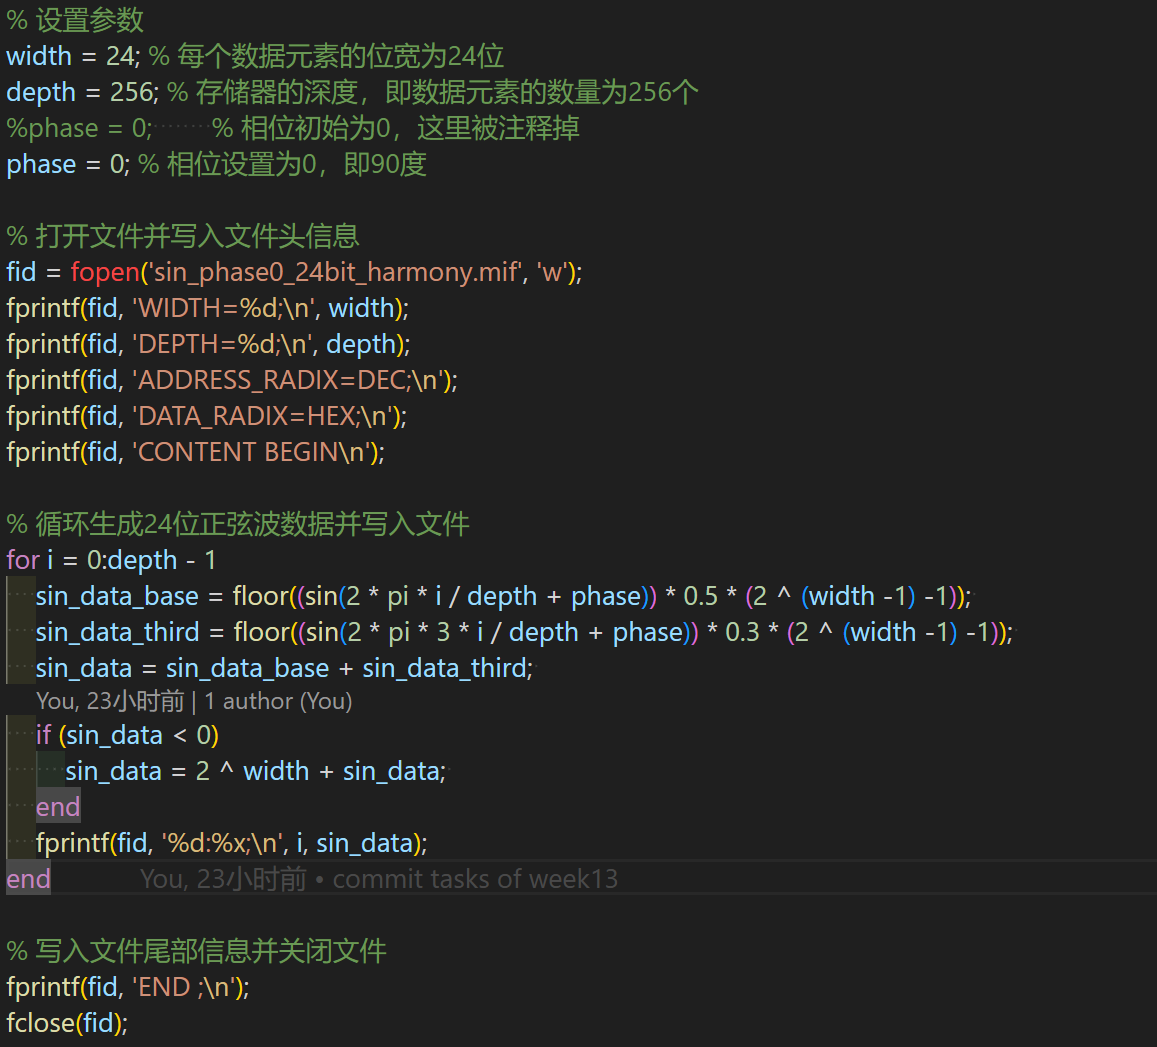
\includegraphics[width=0.8\textwidth]{matlab1.png}
    \caption{matlab代码}
    \label{fig:matlab1}
\end{figure}

最终示波器上显示的波形如图\ref{fig:scope1}所示。
\begin{figure}[!ht]
    \centering
    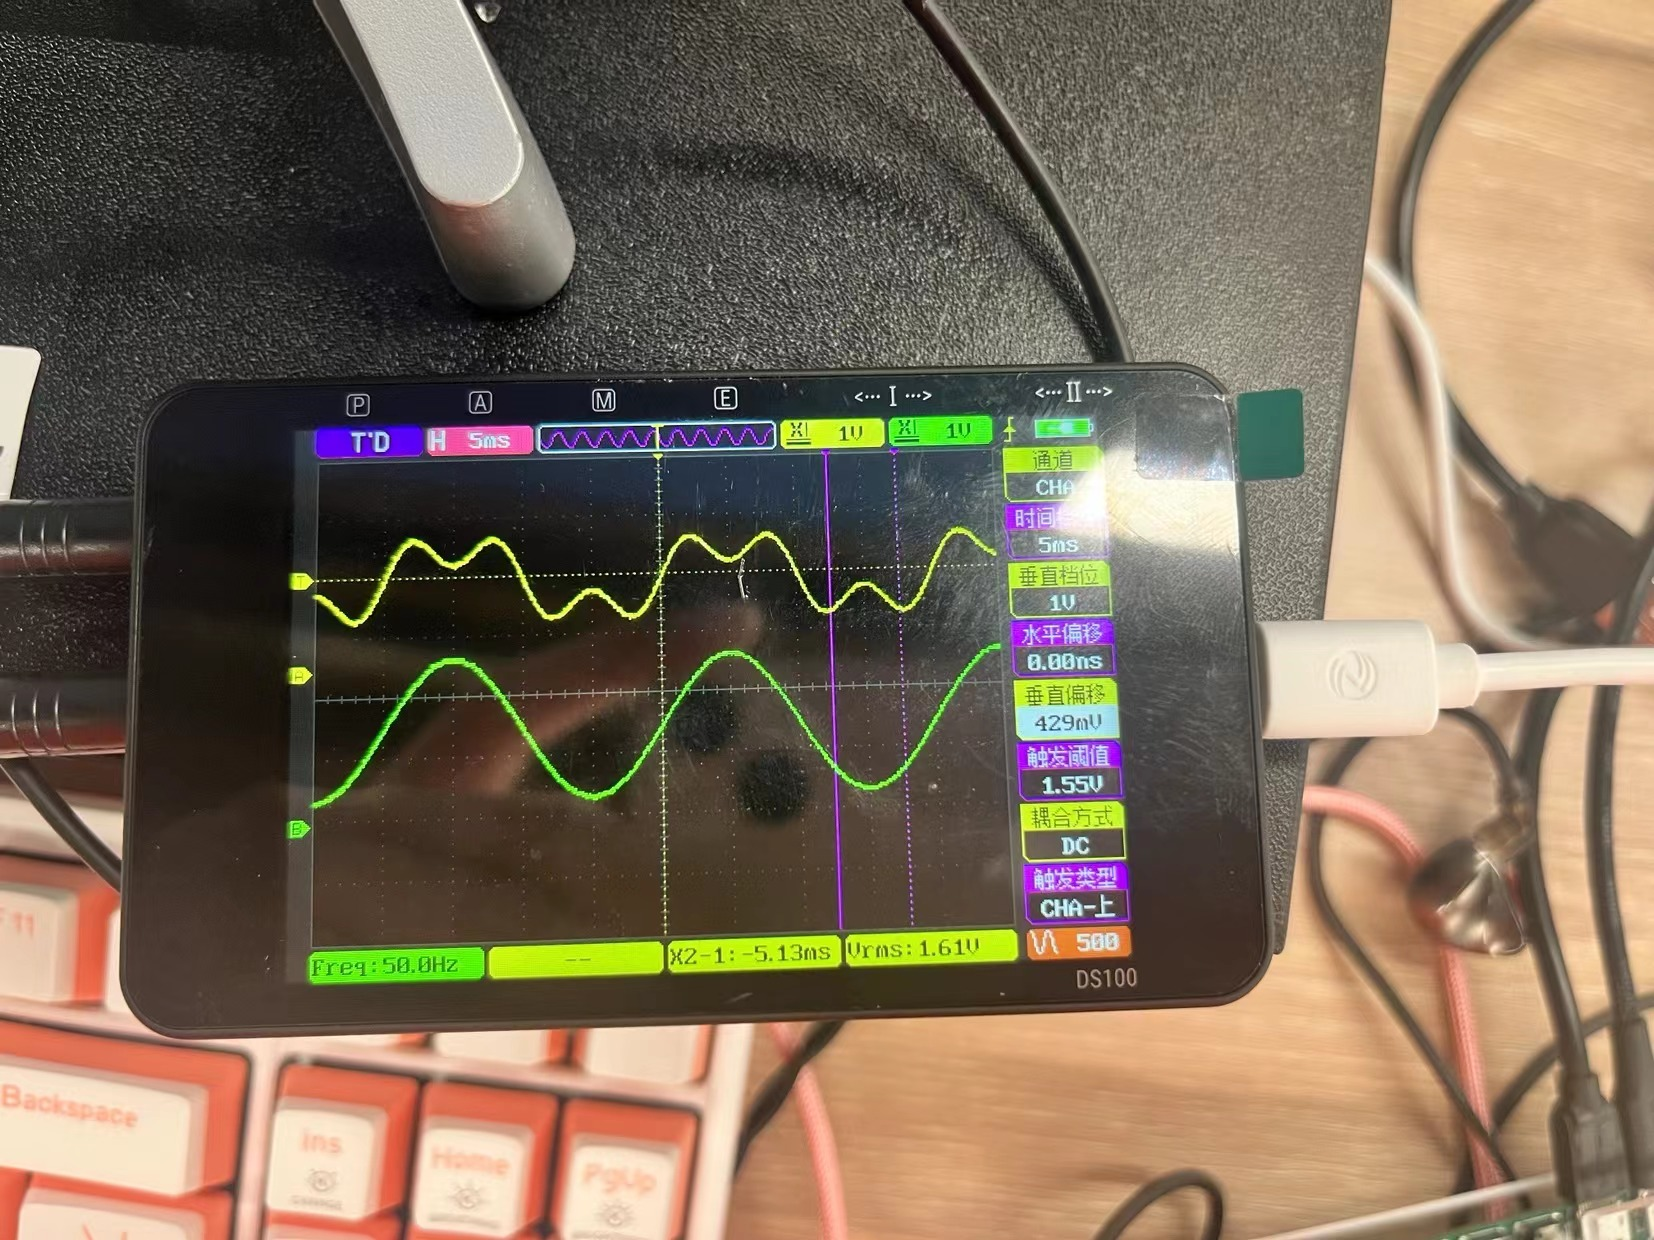
\includegraphics[width=0.8\textwidth]{scope1.png}
    \caption{50Hz正弦波与三次谐波波形}
    \label{fig:scope1}
\end{figure}

\section{task2}
本任务所涉及代码均已在网络学堂给出或在其他任务完成,因此只需给出顶层文件如下:
\begin{framed}
    \begin{lstlisting}[style=verilogStyle]
`include "rom_data_tri.v"
`include "rom_base.v"
`include "rom_harmony.v"
`include "dac_controller_new_1213.v"
`include "mypll2.v"
`include "adc_controller_new_1213.v"

module task2_top(
    input clk,
    input rst,
    input sdout_adc,
    output lrck_dac,
    output sclk_dac,
    output mclk_dac,
    output sdata_dac,
    output mclk_adc,
    output sclk_adc,
    output lrck_adc,
    output reg  buzz,
    output [23:0] dataL_adc,
    output [23:0] dataR_adc
);

initial begin
    buzz = 1'b1;
end

wire[23:0] data_dac_chL;
wire[23:0] data_dac_chR;
wire[7:0] addr_chL;
wire[7:0] addr_chR;
wire c0;//6553600hz
wire c1;//1.28Mhz

rom_data_tri uut1(
    .lr_ch_tri_clk(lrck_dac),
    .rst(rst),
    .addr_chL(addr_chL),
    .addr_chR(addr_chR)
);

rom_base uut2(
    .clock(clk),
    .address(addr_chL),
    .q(data_dac_chL)
);

rom_harmony uut3(
    .clock(clk),
    .address(addr_chR),
    .q(data_dac_chR)
);

dac_controller_new_1213 uut4(
    .clk(c0),
    .rst(rst),
    .data_dac_chL(data_dac_chL),
    .data_dac_chR(data_dac_chR),
    .mclk_dac(mclk_dac),
    .sclk_dac(sclk_dac),
    .lrck_dac(lrck_dac),
    .sdata_dac(sdata_dac)
);

adc_controller_new_1213 uut6(
    .clk(c1),
    .rst(rst),
    .sdout_adc(sdout_adc),
    .mclk_adc(mclk_adc),
    .sclk_adc(sclk_adc),
    .lrck_adc(lrck_adc),
    .dataL_adc(dataL_adc),
    .dataR_adc(dataR_adc)
);

mypll2 uut5(
    .inclk0(clk),
    .c0(c0),
    .c1(c1)
);

endmodule
    \end{lstlisting}
\end{framed}

对应的RTL电路图如图\ref{fig:rtl2}所示。
\begin{figure}[!ht]
    \centering
    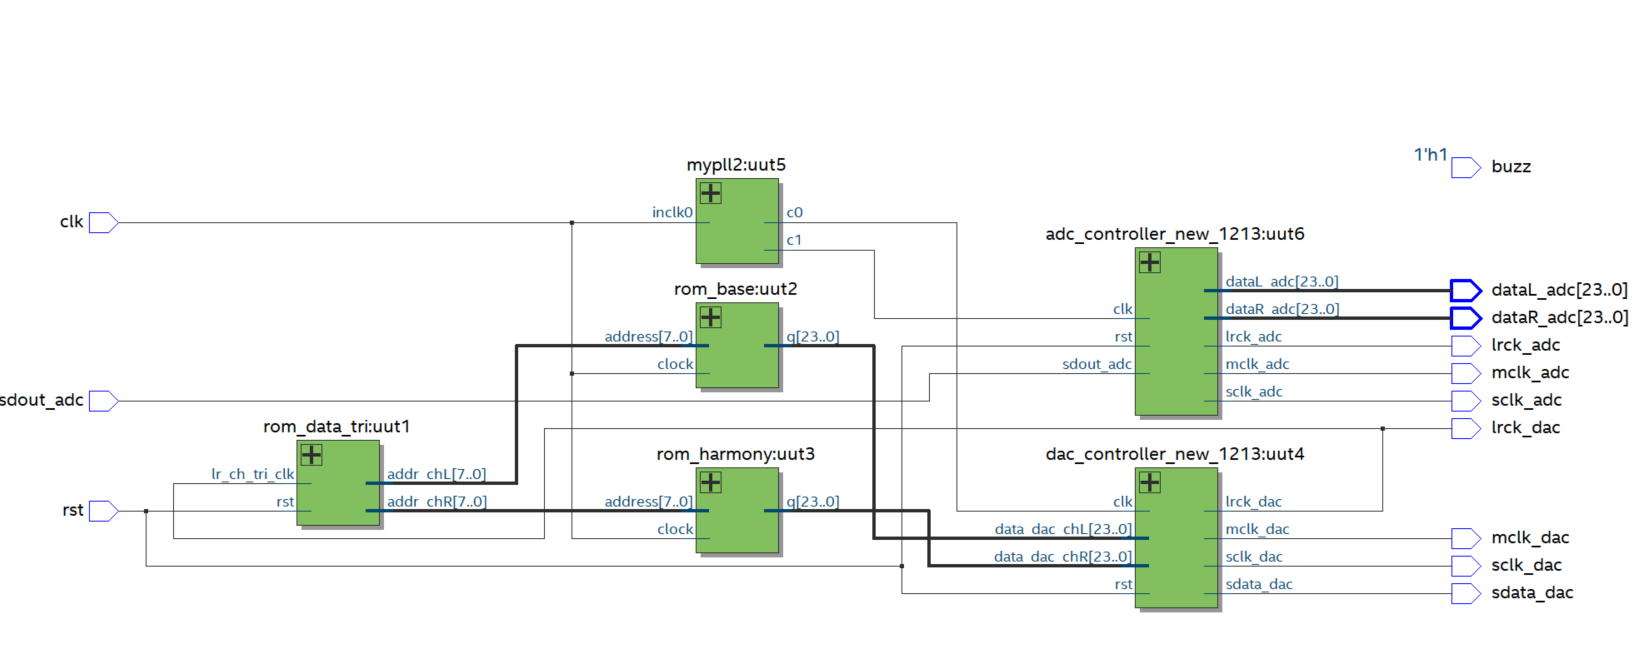
\includegraphics[width=0.8\textwidth]{rtl2.png}
    \caption{task2RTL电路图}
    \label{fig:rtl2}
\end{figure}
\FloatBarrier

通过signaltap观察到的波形如图\ref{fig:signaltap2}所示。
\begin{figure}[!ht]
    \centering
    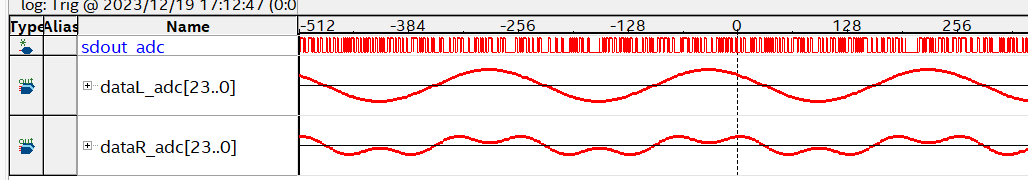
\includegraphics[width=0.8\textwidth]{signaltap2.png}
    \caption{signaltap波形}
    \label{fig:signaltap2}
\end{figure}
\FloatBarrier
\section{task3}
本任务所涉及代码均已在网络学堂给出或在其他任务完成,因此只需给出顶层文件如下:
\begin{framed}
    \begin{lstlisting}[style=verilogStyle]
`include "rom_data_tri.v"
`include "rom_base.v"
`include "rom_harmony.v"
`include "dac_controller_new_1213.v"
`include "mypll2.v"
`include "adc_controller_new_1213.v"
`include "adc_data_ready_tri.v"
`include "uart_NbyteTran_3byteData_controller.v"
`include "uart_tx_byte.v"

module task3_top(
    input clk,
    input rst,
    input sdout_adc,
    output lrck_dac,
    output sclk_dac,
    output mclk_dac,
    output sdata_dac,
    output mclk_adc,
    output sclk_adc,
    output lrck_adc,
    output reg  buzz,
    output [23:0] dataL_adc,
    output [23:0] dataR_adc,
    output  send_en,
    output sci_tx
);

initial begin
    buzz = 1'b1;
end

wire[23:0] data_dac_chL;
wire[23:0] data_dac_chR;
wire[7:0] addr_chL;
wire[7:0] addr_chR;
wire c0;//6553600hz
wire c1;//1.28Mhz

wire tx_done;
wire tx_en;
wire [23:0] data;
wire [7:0] tx_d;
wire send_done;

rom_data_tri uut1(
    .lr_ch_tri_clk(lrck_dac),
    .rst(rst),
    .addr_chL(addr_chL),
    .addr_chR(addr_chR)
);

rom_base uut2(
    .clock(clk),
    .address(addr_chL),
    .q(data_dac_chL)
);

rom_harmony uut3(
    .clock(clk),
    .address(addr_chR),
    .q(data_dac_chR)
);

dac_controller_new_1213 uut4(
    .clk(c0),
    .rst(rst),
    .data_dac_chL(data_dac_chL),
    .data_dac_chR(data_dac_chR),
    .mclk_dac(mclk_dac),
    .sclk_dac(sclk_dac),
    .lrck_dac(lrck_dac),
    .sdata_dac(sdata_dac)
);

adc_controller_new_1213 uut6(
    .clk(c1),
    .rst(rst),
    .sdout_adc(sdout_adc),
    .mclk_adc(mclk_adc),
    .sclk_adc(sclk_adc),
    .lrck_adc(lrck_adc),
    .dataL_adc(dataL_adc),
    .dataR_adc(dataR_adc)
);

mypll2 uut5(
    .inclk0(clk),
    .c0(c0),
    .c1(c1)
);

adc_data_ready_tri uut7(
    .clk(clk),
    .rst(rst),
    .lrck(lrck_adc),
    .send_en(send_en)
);

uart_NbyteTran_3byteData_controller uut8(
    .clk(clk),
    .rst(rst),
    .send_en(send_en),
    .data(dataR_adc),
    .tx_d(tx_d),
    .tx_en(tx_en),
    .tx_done(tx_done)
);

uart_tx_byte uut9(
    .clk(clk),
    .rst(rst),
    .rx_d(tx_d),
    .tx_en(tx_en),
    .tx_done(tx_done),
    .sci_tx(sci_tx)
);
endmodule
    \end{lstlisting}
\end{framed}

对应的RTL电路图如图\ref{fig:rtl3}所示。
\begin{figure}[!ht]
    \centering
    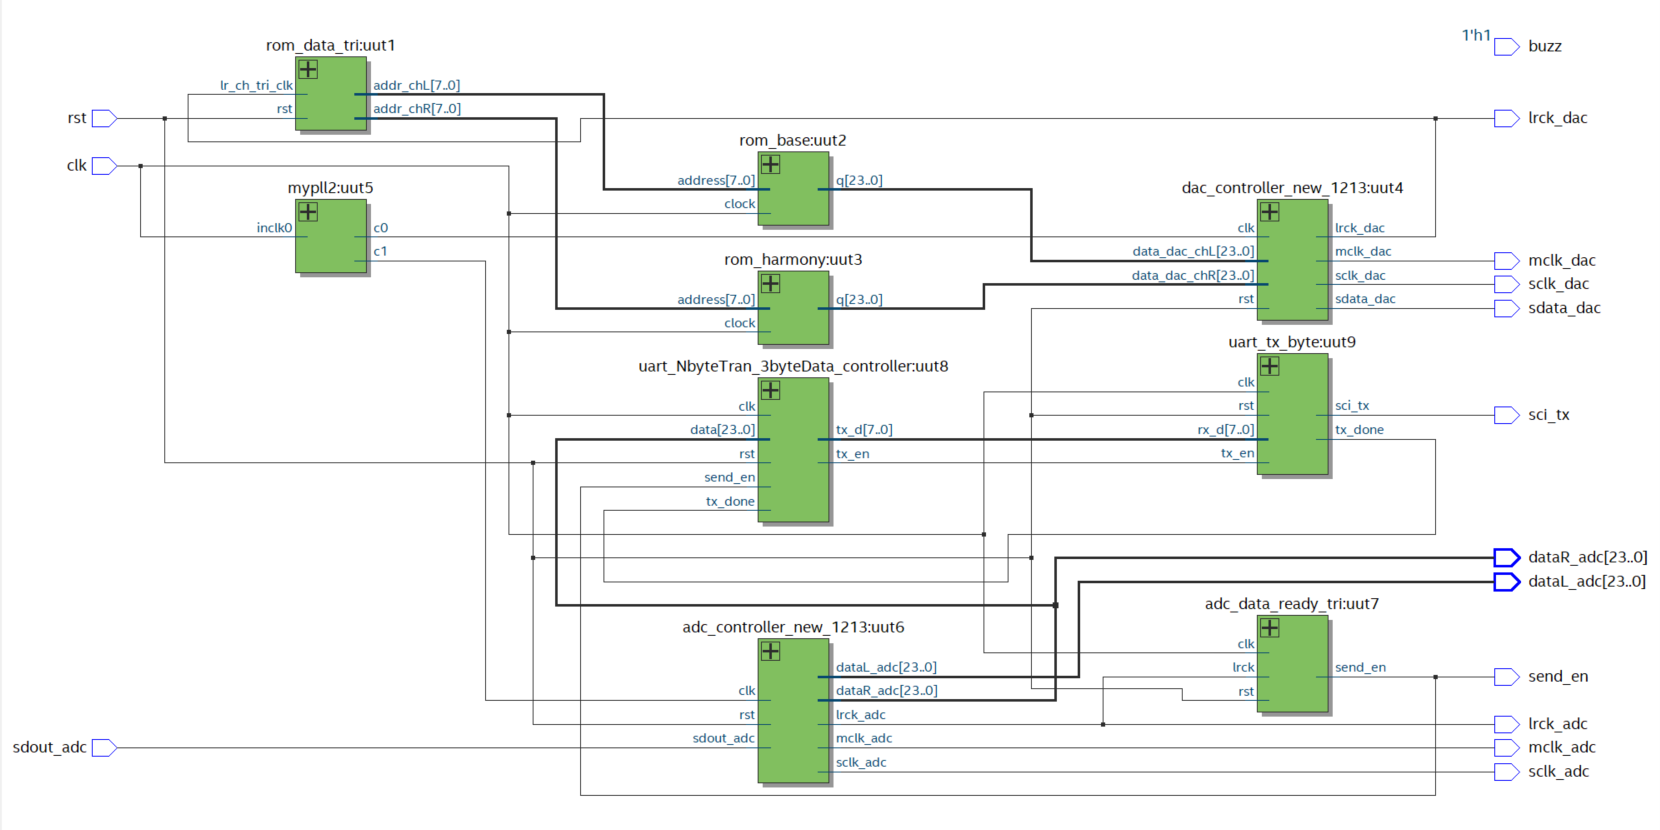
\includegraphics[width=0.8\textwidth]{rtl3.png}
    \caption{task3RTL电路图}
    \label{fig:rtl3}
\end{figure}
\FloatBarrier

simulink设置如图\ref{fig:simulink3}所示。
\begin{figure}[!ht]
    \centering
    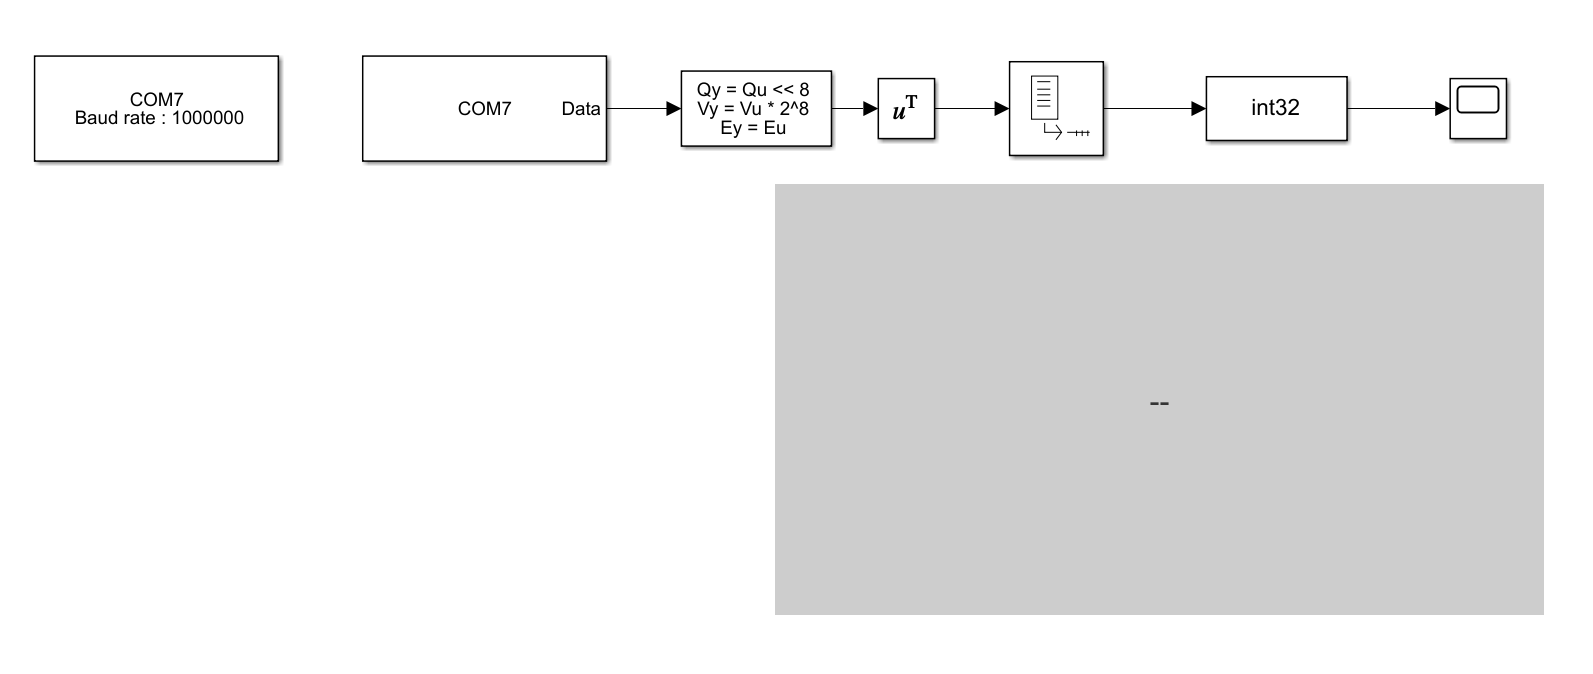
\includegraphics[width=0.8\textwidth]{simulink3.png}
    \caption{simulink设置}
    \label{fig:simulink3}
\end{figure}
\FloatBarrier

simulink接受到的波形如图\ref{fig:scope3}所示。
\begin{figure}[!ht]
    \centering
    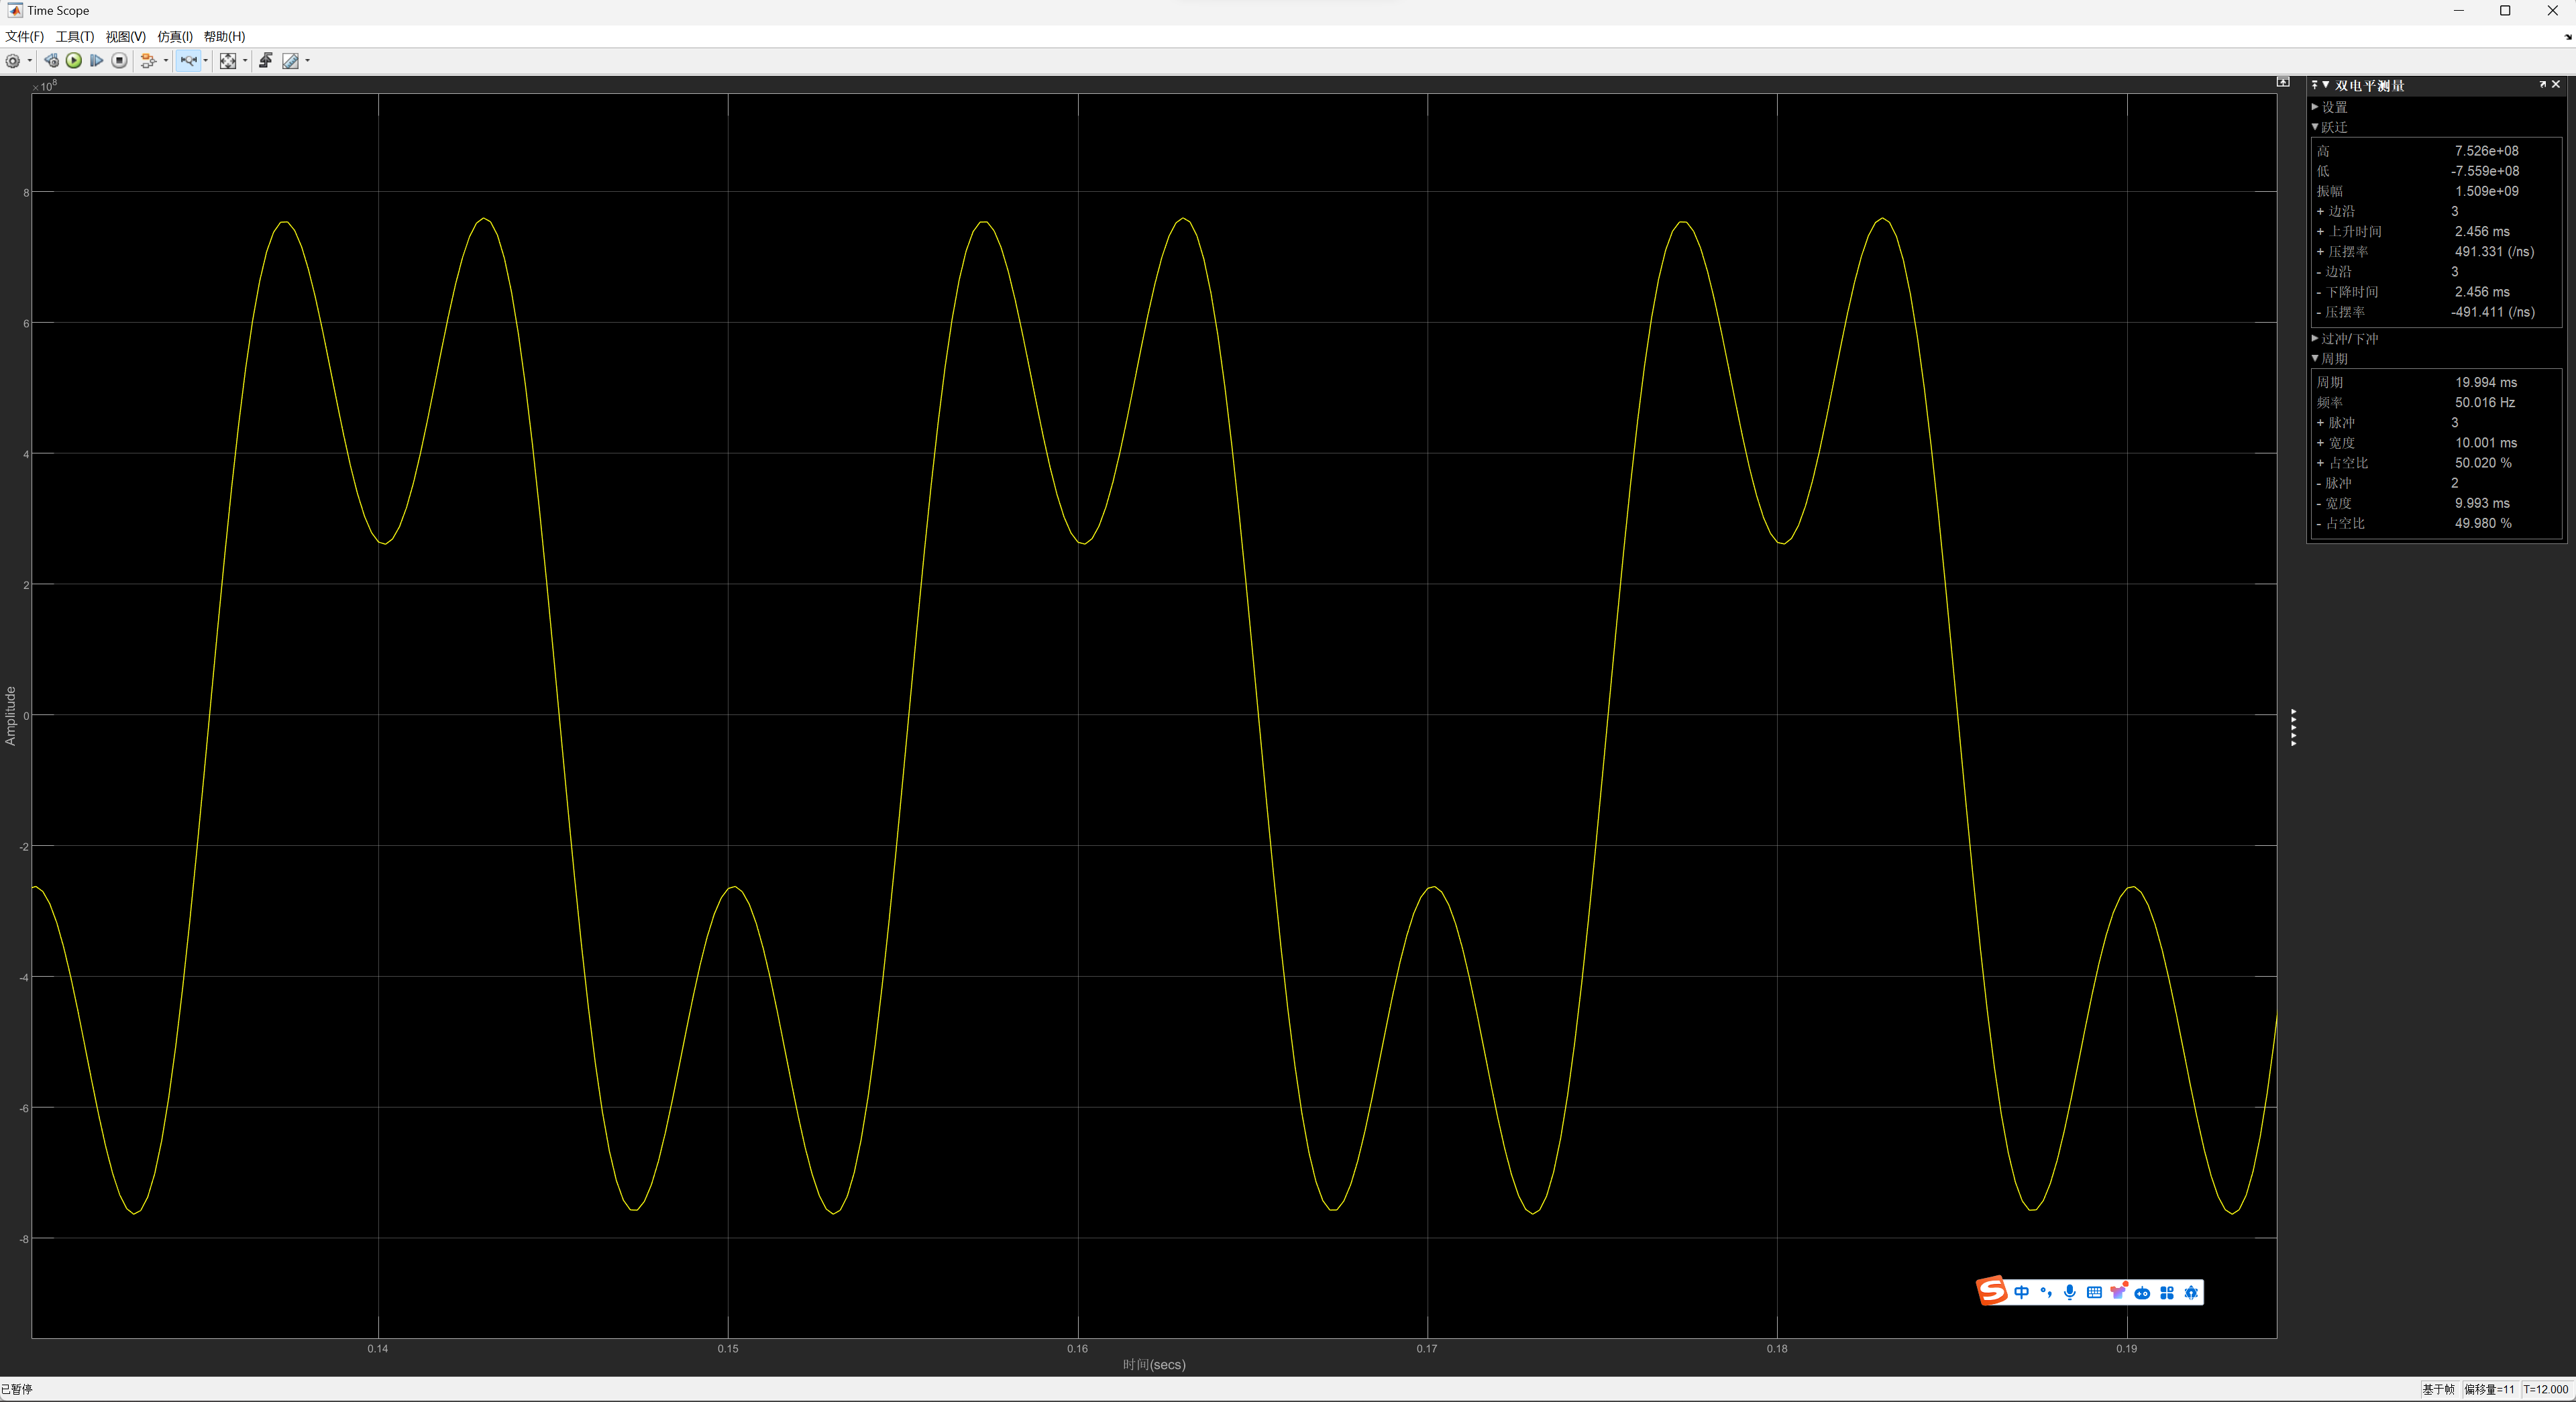
\includegraphics[width=0.8\textwidth]{scope3.png}
    \caption{simulink接受到的波形}
    \label{fig:scope3}
\end{figure}
\end{document}